\chapter{CodeBlue System Evaluation}
\label{chap-eval}
\label{chap-deploy}

This chapter presents evaluation of our CodeBlue prototype. 
The goal is to validate its overall robustness and scalability with multiple
transmitters and receiving devices and to identify the limitations
of our architecture and prototype. We also wish to explore the effect of
increasing data rates on throughput. We present two evaluation studies: one
with an indoor testbed environment and the other as part of a disaster
response drill deployment.

\section{Testbed Evaluation}
\label{sec-cb-eval}
\label{sec-cb-testbed-eval}

We first evaluate our CodeBlue prototype on
MoteLab\cite{motelab-spots05}, an indoor testbed of 30~MicaZ motes,
distributed over 3~floors of Maxwell Dworkin Laboratory.
We measure communication reliability and throughput under a wide range
of link conditions and data rates. We also demonstrate the use of
CodeBlue with mobile receivers.
Our results are promising and show that CodeBlue achieves good packet
delivery ratios with modest data rates. 


\subsection{Evaluation environment}

We use MoteLab testbed to evaluate our CodeBlue prototype. It consisted of 30
MicaZ motes at the time the experiments.  MoteLab forwards messages to and
from each mote's serial port via a TCP socket, allowing us to control and
monitor the entire network from a single machine. We implemented a Java-based
driver to set test parameters and retrieve statistics without having to
reprogram the motes for each experiment. 

In each experiment, we used {\em virtual} sensors on each patient device
that generate data at a constant rate. We used 60 byte packets and the
standard TinyOS MAC, an implementation of CSMA. In order to avoid
start-up effects, we ignore the first and last 60~seconds of each run. 
For data rates below 5~Hz, we ran the experiment for a duration long
enough to produce 200 samples after the first 60 seconds. For higher data
rates, we ran each experiment for three minutes. Therefore, we collect between
200 and 3000~samples per run. 


\subsection{Scalability}

\pic{width=.6\hsize}{./resources/codeblue-nsdi06/figures/eval/warmup/varyDistance.pdf}{\small 
{\bf The effect of increasing data rate and hop count on reception
ratio.} {\em This experiment measures three separate sender-receiver
pairs with different number of radio hops in the routing path. Increasing
the transmission rate leads to degradation in reception ratio due to
dropped packets.}}{fig-eval-varyDistance}

The first set of experiments attempts to answer three 
scalability-related questions about our system:
\begin{itemize}
\item What is the effect of increasing the data rate generated
by each sensor device?
\item What is the effect of increasing the number of senders?
\item What is the effect of increasing the number of receivers?
\end{itemize}
Because of the limited size of our testbed, we are unable to directly 
generate data for very large networks (hundreds of nodes or more).
However, we can emulate this behavior by increasing the
data rate from each transmitter.

\begin{figure}[t]
\begin{center}
\begin{tabular}{cc}
\includegraphics[width=0.45\hsize]{./resources/codeblue-nsdi06/figures/eval/warmup/varyNumSenders.pdf}
& 
\includegraphics[width=0.45\hsize]{./resources/codeblue-nsdi06/figures/eval/warmup/throughput1recv.pdf}
\\
{\small\bf (a) Reception ratio} & {\small\bf (b) Aggregate throughput} \\
\end{tabular}
\end{center}
\caption{\small {\bf Effect of increasing data rate and number of
senders with 1~receiver.} 
{\em Reception ratios are very high for data rates below 5~packets per second, 
even with 10~separate senders over multi-hop paths (1-5 hops).}}
\label{fig-eval-varyNumSenders}
\end{figure}

\paragraph*{Varying data rate and hop count:}
Figure~\ref{fig-eval-varyDistance} shows the packet reception ratio
for three separate sender-receiver pairs. In all three cases, the same
node is used as the sender, while the receiving node is varied. The
receivers were selected to vary the number of radio hops along the
ADMR path. Note that the hop count varies over time because ADMR
routes are dynamic. The single-hop case is very common in clinical
settings where a doctor or nurse is near the patient, while multi-hop
is more likely in a large scale disaster response scenario.

As the figure shows, the reception ratio is very good in the
single-hop case, even for extremely high data rates: 50~packets per
second. With multi-hop, the reception ratio degrades substantially.
There are three reasons that factor into this degradation. First, in
multi-hop routes, forwarding nodes compete for bandwidth with both the
upstream and downstream forwarders, limiting the per-node
bandwidth. This can cause packet queues on some nodes to fill,
eventually forcing packets to be dropped. We instrumented our code to
detect this; however, we never observed dropped packets caused by 
queues filling up.

A second factor is simply the unreliable nature of wireless networks.
As the number of hops in a path increases, more packets get
lost, even without contention. Since packets take
far less than one second to travel from source to destination (see
Section~\ref{sec-cb-latency}), this is the primary effect observed at the
leftmost points on the graph. Thus, for the 5-6 hop path in the
graph, the best we can hope to do without retransmissions is about
63\%.

The last factor is collisions between packets. Because TinyOS uses a
CSMA MAC protocol, which is known to suffer from hidden-terminal
effects \cite{stallings-wireless}, there will be collisions when many
packets are present in the network. Based on our latency measurements
(Section~\ref{sec-cb-latency}), we estimate that at a 50 packet per
second transmission rate there will be 4 or 5 packets in flight at any
given time for the 5-6 hop path. Thus, the decrease in reception
ratio between 1~Hz and 50~Hz is due to collisions. This suggests that
a different MAC protocol may be beneficial.

\begin{figure}[t]
\begin{center}
\begin{tabular}{cc}
\includegraphics[width=0.45\hsize]{./resources/codeblue-nsdi06/figures/eval/warmup/varyNumSenders3.pdf}
& 
\includegraphics[width=0.45\hsize]{./resources/codeblue-nsdi06/figures/eval/warmup/throughput3recv.pdf}
\\
{\small\bf (a) Reception ratio} & {\small\bf (b) Aggregate throughput}\\
\end{tabular}
\end{center}
\caption{\small {\bf Effect of increasing data rate and number of
senders with 3~receivers.} {\em Increasing the number of receiving nodes
has a more serious effect on the reception ratio as data rates are
increased. (Path hop counts in this test ranged from 1 to 7).}}
\label{fig-eval-varyNumSenders3}
\end{figure}

\paragraph*{Varying number of senders:}
Apart from varying the data rate for each sender, we can explore the
effect of varying the number of senders. In each case we use the same
receiving node but increase the number of senders from 1~to~10, and
increase the {\em per-sender} data rate from 1~to~50~packets per
second. In the single-sender case the receiver is within radio range,
but in the other cases the senders are between 1 and 4 hops away. It
is worth noting that as we add senders, the average hop count
increases, so we expect throughput to degrade more rapidly.

The results shown in Figure~\ref{fig-eval-varyNumSenders} are
encouraging: for low data rates (below 5~packets per second per
sender), the reception ratio is above 62\%, even with
10~senders. Given that many vital sign sensors only transmit data at
most once a second, this suggests that the system could scale to a
large number of devices.

\paragraph*{Varying number of receivers:}
We repeated these experiments with 3~separate receivers, using the
same set of senders; Figure~\ref{fig-eval-varyNumSenders3} presents
our results. Because the receivers are no longer within one hop from
the first sender, even in the single sender case we see some
degradation as the data rate increases.
Figure~\ref{fig-eval-varyNumSenders3}(b) shows that the maximum
aggregate bandwidth of 10 senders and 3 receivers is 120~Kbps, or
40~Kbps per receiver. This is consistent with tests that we have
performed measuring the single-hop throughput of Telos motes with the
standard TinyOS CC2420 radio stack. These numbers are far below the
nominal IEEE 802.15.4 channel capacity of 250~Kbps due to MAC and protocol
overheads.

It is worth noting that the reception ratio degradation 
with 3~receivers is much less than what we would expect with
{\em unicast} paths between senders and receivers. 
To get an idea of what the latter case would entail,
consider the reception ratio for 10~senders and 1~receiver in
Figure~\ref{fig-eval-varyNumSenders}(a).
If the sender is generating data at a rate of 10~packets per second and 
relaying data to 3~receivers via unicast, this is roughly equivalent 
to the node generating data at 30~packets per second, 
which results in a reception ratio of about 20\%. However,
the multicast case (Figure~\ref{fig-eval-varyNumSenders3}(a))
shows that with 10~senders, 3~receivers, and a per-sender data 
rate of 10~packets per second, we achieve a reception ratio closer to 40\%. 
This shows that multicast routing in CodeBlue helps mitigate the effects of 
bandwidth limitations.

\subsection{Fairness}

\pic{width=.6\hsize}{./resources/codeblue-nsdi06/figures/senderRecvVsRecpRatio.pdf}{\small
{\bf Fairness across multiple sender-receiver pairs.} {\em This graph shows
the reception ratio breakdown across 18~sender-receiver pairs with
a data rate of 1~packet per second.}}{fig-eval-fairness10}

In a multicast environment with multiple publishers and subscribers,
we are concerned with the overall {\em fairness} achieved by the
routing substrate. If the network unfairly biases certain paths over
others, a doctor receiving data from the system has little confidence
that the data received is evenly distributed across patient sensors.

To demonstrate the overall fairness of the CodeBlue routing layer we
ran an experiment with 3~receivers and 6~senders, each generating data
at a rate of 1~packet per second. We observed that the path lengths
varied between 1~and~6 hops. Figure~\ref{fig-eval-fairness10} shows the
reception ratio breakdown across each sender-receiver pair. As the
figure shows, the reception ratio across all pairs is roughly
equivalent, with a mean of 83\% and a standard deviation of~12\%. In
only one case was the reception ratio less than 60\%.

\subsection{Latency and jitter}
\label{sec-cb-latency}

\begin{figure}[t]
\begin{center}
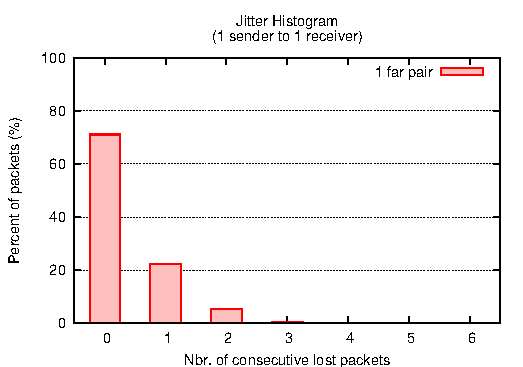
\includegraphics[width=.6\hsize]{./resources/codeblue-nsdi06/figures/jitter1Send1RecvFar.pdf}
\end{center}
\caption{{\small 
{\bf Packet jitter distribution for a single node pair.}
{\em The sender and receiver are placed at opposite ends of the 
building with an average path hop count of 5.}}}
\label{fig-jitter1Send1RecvFar}
\end{figure}

\begin{figure}[t]
\begin{center}
\includegraphics[width=.6\hsize]{./resources/codeblue-nsdi06/figures/jitter6Send3Recv.pdf}
\end{center}
\caption{{\small {\bf Packet jitter distribution across 
6 senders and 3 receivers.} {\em This graph shows packet jitter
for 3~cases: a single-hop node pair, a multi-hop pair, and
across all 18~node pairs.}}}
\label{fig-jitter6Send3Recv}
\end{figure}

The scalability results show that bandwidth limitations are a serious
issue in CodeBlue. Apart from reduced
packet reception ratios, we are concerned about the potential
impact on packet {\em latency} induced by background traffic.
In addition, we are interested in studying the pattern of packet
loss; that is, whether losses occur in large bursts or more intermittently.

\paragraph*{Latency:}
Measuring packet latency in a multi-hop network is difficult and would 
require either fine-grained time synchronization between senders and 
receivers or a round-trip latency measurement. Time synchronization
using a protocol such as FTSP~\cite{ftsp} is possible, although the
results would depend on FTSP's accuracy in our testbed.
Round trip measurements are problematic in the ADMR framework 
because different paths would be chosen in the forward and reverse 
directions. 

Instead, we chose to instrument the message path in CodeBlue by having
senders, receivers, and forwarders send debug messages to their serial
ports during the routing process. These messages are received by the
central testbed server and timestamped with an accuracy of
milliseconds; however, because this time stamping involves several
context switches on the (loaded) server it is only used to derive an
upper bound on the latency.

We measured the end-to-end latency for several multi-hop paths of up
to 7 hops at a data rate of 1 packet per second. In all cases, the
end-to-end message delay was less than 200~ms. Through link-level
measurements in our testbed, we have measured the MAC delay of the
TinyOS radio stack under a wide range of traffic conditions. The
delay varies between 3~ms with no background traffic to about 15~ms
with heavy background traffic. We believe this range generally
characterizes expected per-hop packet latencies in the CodeBlue
environment.

\paragraph*{Packet jitter:}
We define {\em packet jitter} as the number of consecutive dropped
packets for a given sender-receiver pair. This can be measured by
comparing packet sequence numbers on the receiver. If the jitter were
very large, we would be concerned that much critical medical data
would be lost. Figure~\ref{fig-jitter1Send1RecvFar} shows a histogram
for a single sender-receiver pair placed at an average distance of
5~hops. As the figure shows, the packet reception ratio is about
70\%. In 22\% of the cases, the jitter was equal to 1; in less than
8\% of the cases the jitter is 2 or more packets. In no case was a
jitter of more than 5~packets observed.

To understand how multiple senders and receivers affect packet jitter,
we repeated the previous experiment with 6 senders and 3 receivers
distributed throughout the building, transmitting one packet per
second. Figure~\ref{fig-jitter6Send3Recv} shows the jitter histogram
for all 18~pairs. The figure also shows the jitter for two specific
paths: the multi-hop pair from our previous experiment with 1 sender
and 1 receiver, and a single-hop pair. No jitter is observed for 86\%
of the packets, 9\% of packets experienced a jitter of 1, and 5\% of
the packets experienced a jitter greater than 1. The maximum jitter
observed in this case was 23~packets. It is interesting to note that
with multiple senders and receivers, jitter is reduced for the first
pair of nodes (the same pair that was measured in
Figure~\ref{fig-jitter1Send1RecvFar}). This is explained by the
increased number of forwarders, which increases the chance of packets
getting through. The jitter performance suggests that when the number of
sender receiver pairs is small, best-effort delivery suffices to
support applications that can tolerate a few consecutive packet
losses. As the number of communicating pairs grow, worst case jitter
becomes serious and should be be fixed by providing some level of
reliability at the routing layer. CodeBlue, as an architecture, does
not require such reliability but is flexible enough that a reliable
protocol can be implemented without impacting the other components in
the system.



\subsection{Effect of mobility}

\pic{width=.6\hsize}{./resources/codeblue-nsdi06/figures/mobility.pdf}{\small
  {\bf Effect of mobility.} {\em Reception ratio averaged over 60
  second intervals for 3 senders and a single roaming 
  receiver.}}{fig-eval-mobility}

The next evaluation that we present concerns the impact of
mobility on communication reliability. As senders or receivers move in
a hospital, radio link quality will vary and the routing layer will create new
routes. Ideally a valid route is maintained at all times.

In this experiment, we configured 3~fixed nodes as patient sensors
transmitting data at 5 packets per second. The senders were widely
distributed throughout the building. A single receiver node attached to a
laptop acted as a roaming node. The user carrying the laptop
moved around the second floor of our building at a normal walking
pace, pausing occasionally, entering and leaving rooms, for a
duration of about 25~minutes. This movement pattern was intended
to represent a doctor walking through a hospital ward.

Figure~\ref{fig-eval-mobility} shows the reception ratio for each of
the 3 senders, averaged over 60 second windows. As the receiver walks
around, we see the reception ratios vary over time, but do not see any
large dropouts or catastrophic effects due to mobility. We also
recorded the hop count and ADMR path cost for each packet and see a
general correlation between improved delivery ratio and reduced path
cost. These results show that ADMR deals gracefully with node
movement, at least for {\em typical} mobility rates.


\subsection{Mitigating packet loss}

\begin{figure}[t]
\begin{center}
\includegraphics[keepaspectratio,width=.6\hsize]{./resources/codeblue-nsdi06/figures/eval/warmup/kTransmit.pdf}
\end{center}
\caption{\small
  {\bf Mitigating packet loss by transmitting each message multiple times.} {\em Data is shown for a single multi-hop path.}}
\label{fig-eval-ktransmit}
\end{figure}

Although our prototype does not currently provide a reliable routing
mechanism, we anticipate that reliable communication will be necessary
for many medical scenarios, especially for clinical studies and for
alert messages during patient monitoring. Our focus has been
on unreliable multicast, which allows the system to scale to many
patient sensors and receiving devices.

We wish to emphasize that not all medical data needs to be delivered
with 100\% reliability: a doctor or nurse receiving periodic vital
sign updates from a set of patients can tolerate some amount of
intermittent data loss, as long as the loss is not persistent and is
distributed uniformly over the set of patients being monitored.
However, certain signals, such as alerts from critically ill patients
or high-resolution EKG traces, must be delivered with stronger
reliability guarantees. We expect that medical sensor networks will
require a range of reliability semantics from best effort to
guaranteed delivery, depending on the nature of the data. The goal of
the system should be {\em graceful degradation} of communication
reliability under heavy traffic load.

The best approach to implementing reliability is not immediately
clear. Using link-by-link acknowledgment and retransmission with
multicast requires additional MAC support and may incur high overhead.
End-to-end reliability is highly sensitive to overall path conditions.

One simple approach that is worth considering makes use of redundant
transmissions.
We have conducted experiments where each message is
simply transmitted multiple times by the sender. In this way a
receiver can recover the original data if any one of $k$ transmitted
packets is received. Though it consumes considerably more bandwidth,
this approach should yield an estimate of the improvement obtainable
via more sophisticated techniques.

Figure~\ref{fig-eval-ktransmit} shows the result of a series of
experiments with a single multi-hop path with an average path length
of 5 hops. As the figure shows, for low data rates (below 15~packets
per second), using multiple transmissions per packet increases
robustness considerably, from 63\% (with 1~transmission) to over 98\%
(with 5~transmissions). However, at higher data rates the increased
message load causes network saturation and reception ratios drop
considerably. Ideally, nodes would be able to tune their transmission
rates according to background traffic conditions.

\section{Deployment Evaluation}
\label{sec-livenet-deployment-eval}
\label{sec-livenet-deployment}

In addition to evaluating CodeBlue in an indoor controlled environment, we
deployed the system as part of a disaster response drill which took place in
August~2006 in Baltimore, Maryland. During this drill, 10~patients 
were monitored and triaged 
following a simulated bus accident. The network experienced highly variable
performance due to node mobility and a bug, discovered using the LiveNet,
causing massive packet flooding.


\subsection{Disaster Drill}
\label{sec-livenet-drill}

\begin{figure}[t]
\begin{center}
\includegraphics[width=0.6\hsize]{./resources/livenet-sensys07/figs/drill/drill2.pdf}
\end{center}
\caption{\small {\bf The indoor treatment area of the disaster
drill.} {\em Faces are blurred to preserve anonymity. 
Inset shows the electronic triage tag, consisting of an
MSP430 processor, CC2420 radio, status LEDs, display, and 
pulse oximeter for measuring patient vital signs.}}
\label{fig-drill}
\end{figure}

The disaster drill modeled a simulated bus accident in which ten
volunteer ``victims'' were triaged and treated on the scene by 
medics and firefighters participating in the
drill. The patients were outfitted with sensor nodes to
monitor vital signs, which formed an {\em ad-hoc} network, relaying
real-time data back to up to three laptop base stations located near the
incident command post and in an ambulance. The base stations displayed the triage status and vital
signs for each patient, and logged all received data to a file. The
incident commander could rapidly observe whether a given patient required 
immediate attention, as well as update the status of each patient, for
example, by setting the triage status from ``moderate'' to ``severe.''

The network consisted of two types of sensor nodes: an
{\em electronic triage tag} and a {\em electrocardiograph} (EKG).
The triage tag incorporates a pulse oximeter
(monitoring heart rate and blood oxygen saturation using a small
sensor attached to the patient's finger), an LCD display for
displaying vital signs, and multiple LEDs for indicating the patient's 
triage status (green, yellow, or red, depending on the patient's severity). 
The triage tags are based on the MicaZ mote with a custom 
daughterboard and case, as shown in Figure~\ref{fig-drill}. The EKG
node consists of a TMote Sky with a custom sensor board
providing a two-lead (single-channel) electrocardiograph signal that
is digitized by the mote for transmission over the radio. 
In addition to the patient sensor nodes, a number of static repeater
nodes were deployed to assist with maintaining network connectivity.

The sensor nodes were all programmed with an improved version of CodeBlue that supports the
triage tag sensor platform and incorporates an experimental publish/subscribe 
routing protocol, Flows, to support hop-by-hop retransmissions (ARQ). 
The reason for choosing Flows is to improve the packet delivery reliability 
in the CodeBlue network. Similar to TinyADMR, Flows exposes a publish/subscribe
interface, performs flooding based route discovery, and uses PATH-DR as
routing metric. The main difference is that Flows enables link level
acknowledgments (ACK) and retransmits packets up to 5 times if no ACKs are
received from the next hop.


LiveNet was deployed along with the network at the disaster drill site. The
goal was to capture detailed data on the
operation of the network as nodes were activated, patients moved from
the triage to treatment areas, and study the scalability and
robustness of our CodeBlue system. In this
situation, it would have been impossible to record complete packet
traces from each sensor node directly, motivating the need for a
passive monitoring infrastructure. We made use of 7~separate sniffer
nodes attached to 5~laptops (two of the laptops had two~sniffers to
improve yield). 

Figure~\ref{fig-drill} shows a picture from the drill to give a sense
of the setup. The drill occurred in three stages. The first stage
occurred in a parking lot area outdoors during which patients were
outfitted with sensors and initial triage was performed. In the second
stage, the patients were moved to an indoor treatment area
as shown in the picture. In the third stage, two of the ``critical''
patients were transported to a nearby hospital. LiveNet sniffers were
placed in all three locations. Our analysis in this paper focuses on
data from 6~sniffers located at the disaster site.

The drill ran for a total of 53~minutes, during which we recorded a 
total of 110548~packets in the merged trace from a total of
20 nodes (11~patient sensors, 6~repeaters and 3~base stations).



\subsection{General evaluation}
\label{sec-livenet-general-eval}

\begin{figure}[t]
\begin{center}
\includegraphics[width=0.9\hsize]{./resources/livenet-sensys07/figs/drill/rate/drill-rate.pdf}
\end{center}
\caption{\small {\bf Overall traffic rate during the disaster drill.}
{\em The total traffic is averaged over 30~sec windows and
is broken down by type: queries/status packets, query reply
packets, route maintenance packets, and corrupted packets. The broadcast storm
begins at time 10:39.}}
\label{fig-drill-traffic}
\end{figure}

\begin{figure}[t]
\begin{center}
\includegraphics[width=0.6\hsize]{./resources/livenet-sensys07/figs/drill/type/type.pdf}
\end{center}
\caption{\small {\bf Packet type breakdown for a portion of the
disaster drill.} 
{\em The graph shows the sender and type for each packet during a
portion of the disaster drill. Periodic status and route maintenance
messages can be seen along with query replies. Packets with invalid header
fields are also shown; the broadcast storm can be seen starting at 10:39:29.}}
\label{fig-drill-type}
\end{figure}


As a general evaluation of the sensor network's operation during the
drill, we first present the overall traffic rate and packet type
breakdown in Figure~\ref{fig-drill-traffic}~and~\ref{fig-drill-type}.
These high-level analyses help us understand the operation of the
deployed CodeBlue network and can be used to discover performance 
anomalies that are not observable from the network sinks.

As Figure~\ref{fig-drill-traffic} shows, at around time
$t=10:39$ there is a sudden increase in corrupted packets received
by LiveNet: these packets have one or more fields that appear to
contain bogus data. Looking more closely at Figure~\ref{fig-drill-type}, 
starting at this time we see a large number of partially-corrupted
routing protocol control messages being flooded in the network. 
On closer inspection, we found that these packets were otherwise
normal route discovery messages that contained bogus
sequence numbers. This caused the duplicate suppression 
algorithm in the routing protocol to fail, initiating a perpetual
broadcast storm that lasted for the entire second half of the drill.
The storm also appears to have negatively affected application
data traffic as seen in Figure~\ref{fig-drill-traffic}.

We believe the cause to be a bug in the routing protocol (that we
have since fixed) that only occurs under heavy load. Note that we 
had no way of observing this bug without LiveNet, since the 
base stations would drop these bogus packets.

\subsection{Coverage}
\label{sec-livenet-drill-coverage}

\begin{figure}[t]
\begin{center}
\includegraphics[width=0.6\hsize]{./resources/livenet-sensys07/figs/coverage/drill/drill-coverage-bynode.pdf}
\end{center}
\caption{\small {\bf Per-node coverage during the drill.}
{\em This graph shows the coverage of the LiveNet sniffers for
each of the 20~nodes in the disaster drill. Coverage for mobile patient
sensors is lower than for the fixed repeater nodes. The
overall coverage is 58\%.}}
\label{fig-drill-coverage}
\end{figure}

To determine sniffer coverage, we make use of periodic status
messages broadcast by each sensor node once every 15~sec. Each status
message contains the node ID, sensor types attached, and a 
unique sequence number. The sequence numbers allow us to identify gaps
in the packet traces captured by LiveNet, assuming that all
status messages were in fact transmitted by the node. A node could
conceivably fail to transmit a status message due to excessive CSMA
back-off, so the results here are conservative. 

Figure~\ref{fig-drill-coverage} shows the coverage broken down by each
of the 20~nodes in the disaster drill. There were a total of 4819
expected status messages during the run, and LiveNet 
captured 59\% overall. We observed 89~duplicate and
out-of-order packets out of 2924~packets in total, for an error rate of 3\%. 
As the figure shows, the coverage for the fixed repeater nodes is
generally greater than for the patient sensors; this is not too
surprising as the patients were moving between different locations
during the drill, and many patients were laying on the ground.
The low coverage (26\%) for one of the sink nodes is because this node
was located inside an ambulance, far from the rest of the deployment.

\subsection{Topology and network hotspots}
\label{sec-livenet-topology-path}


\begin{figure}[t]
\begin{center}
\includegraphics[width=0.8\hsize]{./resources/livenet-sensys07/figs/topology/drill/topology.pdf}
\end{center}
\caption{\small {\bf Unicast links observed during the disaster drill.}
{\em Data is shown only for the first half of the drill, before all
nodes were moved indoors together. Each edge is labeled with 
the mean number of packet transmissions (ETX) along the link. 
Blue nodes are patient sensors, red nodes are repeaters, 
and green nodes are sinks.}}
\label{fig-drill-topology}
\end{figure}


\begin{figure}[t]
\begin{center}
\includegraphics[width=0.6\hsize]{./resources/livenet-sensys07/figs/hotspot/inferred-hotspot.pdf}
\end{center}
\caption{\small {\bf Inferred per-node packet traffic load during the drill.}
{\em This graph shows the number of packets transmitted 
by each node during the drill. Both observed traffic and inferred traffic
based on sequence number analysis are shown in the graph.}}
\label{fig-drill-hotspot}
\end{figure}

The network topology during the drill was very chaotic, since nodes
were moving and several nodes experienced reboots. Visualizing such a
complex dataset presents challenges of its own, but to give an example
we show the partial topology consisting only of observed unicast links
in Figure~\ref{fig-drill-topology}. The full connectivity graph
including all neighbor relationships is too dense to show here.
For each link, we evaluate the ETX metric~\cite{etx}, 
defined as the mean number of transmissions of a 
given packet along each link; our routing protocol uses ARQ with a
maximum retransmission count of~5. This data can be used to 
estimate radio link quality.

A few observations can be made from this figure. First, most nodes
use several outbound links, indicating a fair amount of route
adaptation. Keep in mind
that there are multiple routing trees (one rooted at each of the sinks), 
and node mobility causes path changes over time.
Second, all but two of the patient sensors have both incoming and outgoing
unicast links, indicating that they were used for relaying packets. We
also see one of the sink nodes (node 100) relaying packets as well. 

In order to determine ``hotspots'' in the network, we look at the
total number of packets transmitted by each node during the drill.
For several message types (query reply and status messages), we can
also infer the existence of unobserved packets using sequence numbers; 
this information is not available for route maintenance and query messages.
Figure~\ref{fig-drill-hotspot} shows the breakdown by node ID and
packet type. Since we are counting all transmissions by a node, these
totals include forwarded packets; this explains the wide variation in 
traffic. 

Figure~\ref{fig-drill-hotspot} reveals a few interesting features. the repeater nodes
generated a larger amount of traffic overall than the patient
sensors; this indicates that the repeaters were heavily used, as
suggested by the topology shown in Figure~\ref{fig-drill-topology}. 
Second, node~62 (a repeater) seems to have a very large number of
inferred (that is, unobserved) query reply packets, far more than its
coverage of 83.6\% would predict. This suggests that the node 
internally dropped packets that it was forwarding
for other nodes, possibly due to heavy load. Note that with 
the information in the trace, there is no way to disambiguate packets 
unobserved by LiveNet from those dropped by a node. If we assume
that our coverage calculation is correct, we would infer
a total of 4088 packets; instead we infer a total of 15017. Node 62 may have
then dropped as many as $(15017-4088)/15017 = 72\%$ of the query 
replies it was forwarding. With no further information, 
the totals in Figure~\ref{fig-drill-hotspot} therefore represent 
a conservative upper bound on the total traffic transmitted by the node.

\subsection{Path inference}

\begin{figure}[t]
\begin{center}
\includegraphics[width=0.9\hsize]{./resources/livenet-sensys07/figs/pathinference/drill/22_104/alpha_01/22_104_route_change_plot.pdf}
\end{center}
\caption{\small {\bf Routing paths for one of the patient
sensors during the disaster drill.}}
\label{fig-drill-path}
\end{figure}

Given the limited coverage of the LiveNet sniffers during the drill,
we would not expect the path inference algorithm to provide results
as crisp as those in Figure~\ref{fig-path-validation}. We take as an
example a single patient sensor (node 22) and infer the routing paths to one of
the sink nodes (node 104). 
The results are shown in Figure~\ref{fig-drill-path}.
As the figure shows, there are many inferred paths that lack complete
observations of every hop, and the $\Pi$ scores for these paths vary
greatly. The path $22 \rightarrow 62
\rightarrow 104$ is most common; node 62 is one of the repeaters.
In several cases the routing path alternates between repeaters 62~and~68.
The node also routes packets through other repeaters, as well as 
several other patient sensors. The longest routing path inferred is 5~hops. 

This example highlights the value of LiveNet in understanding fairly
complex communication dynamics during a real deployment. We were
surprised to see such frequent path changes and number of routing paths
in use, even for a single source-sink pair. This data can help us
tune the routing protocol to better handle mobility and varying link quality.

\subsection{Query behavior and yield}

\begin{figure}[t]
\begin{center}
\includegraphics[width=0.6\hsize]{./resources/livenet-sensys07/figs/drill/query-behavior/query-behavior.pdf}
\end{center}
\caption{\small {\bf Query behavior.} 
{\em This figure shows the behavior of an individual query during the
drill. The plot labels query reply packets received at the sink versus
packets received by the sniffers, indicating packet loss along the
routing path. Sequence number resets can be caused by a query timeout
or a node reboot, also labeled in the figure.}}
\label{fig-drill-query-behavior}
\end{figure}

\begin{figure}[t]
\begin{center}
\includegraphics[width=0.6\hsize]{./resources/livenet-sensys07/figs/drill/query-breakdown/query-breakdown.pdf}
\end{center}
\caption{\small {\bf Query yield per node during the disaster drill.}
{\em The overall data yield during the drill was quite low. Using the
LiveNet infrastructure, we were able to break down the causes of data
loss in terms of packet loss and query timeout.}}
\label{fig-drill-query-yield}
\end{figure}

\begin{figure}[t]
\begin{center}
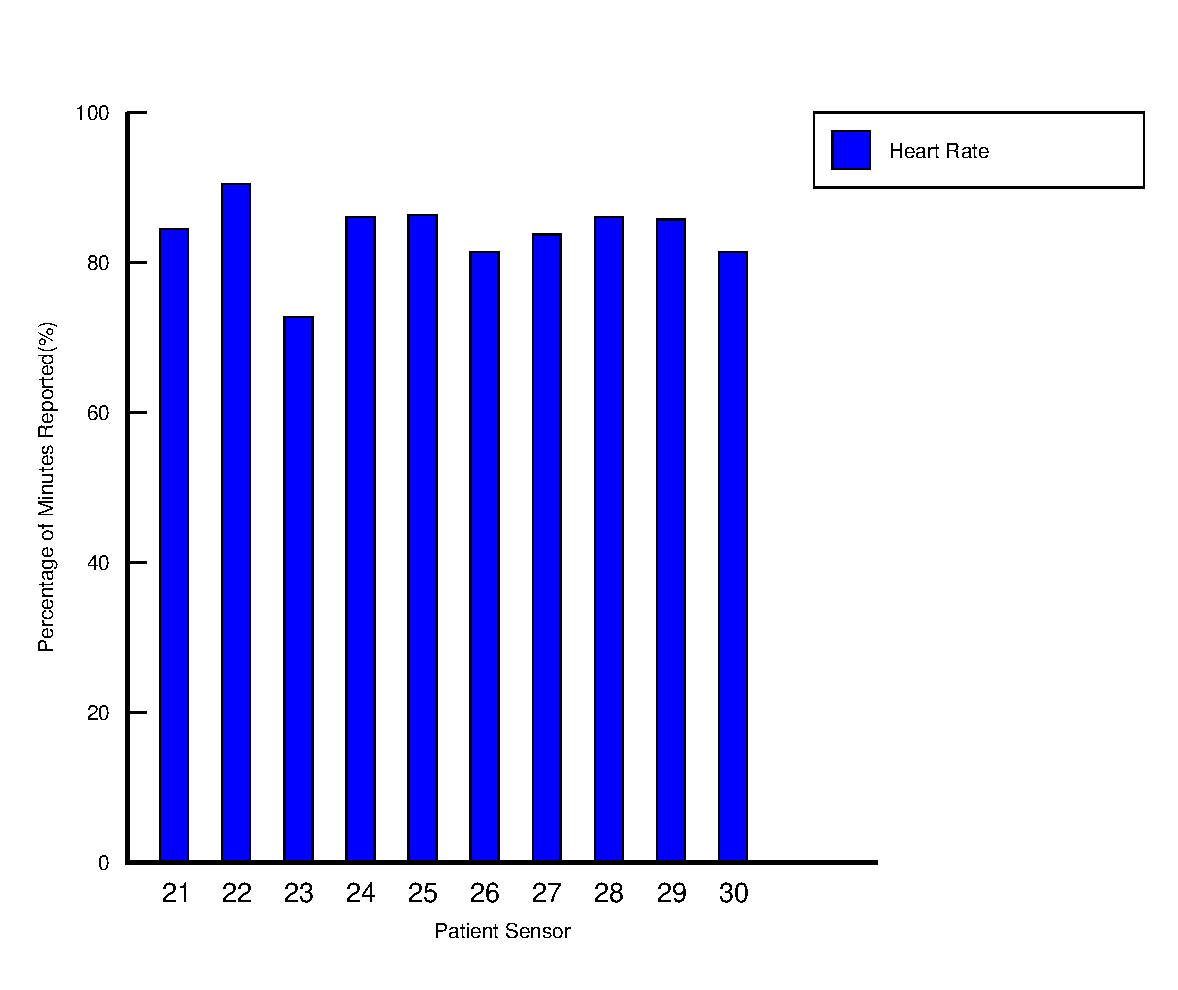
\includegraphics[width=0.6\hsize]{./resources/livenet-sensys07/figs/drill/query-breakdown/query-coverage.pdf}
\end{center}
\caption{\small {\bf Query yield per node when expecting to receive sensor
data every minute.} {\em For this graph, we divide the drill event into
one-minute intervals and present the proportion of the one-mintute intervals
during which our sinks were able to receive the heart rate sensor data. With
this definition, the average yield is 83.83\% across 10 patient sensors.}}
\label{fig-drill-query-coverage}
\end{figure}

The final analysis that we perform on the disaster drill traces
involves understanding the causes of data loss from sources to sinks.
We found that the overall data yield during the drill was very low, 
averaging about 20\% across the patient sensors. 
There are several possible sources of data loss in our system: 
packet loss along routing paths, node failures or reboots, or query
timeout. 


During the drill, most patient nodes ran six simultaneous CBQ queries, 
sending two types of vital sign data at 1~Hz to three sinks.
Each data packet carries a unique sequence number.
Our system uses a lease model for queries, in which the node stops
transmitting data after a timeout period unless the lease is renewed
by the sink. Each sink was programmed to re-issue the query 10~sec before 
the lease expires; however, if this query is not received by the node
in time, the query will time out until the sink re-issues the query.

Figure~\ref{fig-drill-query-behavior} shows the behavior of an
individual node during the drill, combining LiveNet traces with 
base station packet traces collected at the sink nodes. 
From this graph we can infer time periods when queries were active 
or inactive, query timeouts, and path loss to the sink (that is, a packet
observed by LiveNet but not received at the sink). For example, for
the first 100~seconds or so, the node is transmitting packets but none of
them are received by the sink, indicating a bad routing path.

Using this combined information, we can then break down the data loss 
in terms of path loss, inactive query periods (caused by query timeouts), and 
{\em unobserved loss}; that is, packets that were neither observed by
LiveNet or the sink. Figure~\ref{fig-drill-query-yield} shows the results. 
A query yield of 100\% corresponds to the sink receiving packets at
exactly 1~Hz during all times that the node was alive. As the figure
shows, the actual query yield of CodeBlue in this deployment was 17--26\%. Using the
LiveNet traces, we can attribute 5--20\% loss to dropped packets
along routing paths, and 16--25\% loss to premature query timeouts. 
The rest of the loss is unobserved, but likely corresponds to path
loss since these packets should have been transmitted during query
active periods. However, it is also possible that nodes failed to
transmit these packets at all, due to excessive CSMA back-off. 

Even though the overall reliability of CodeBlue seems low for the disaster
drill, partially due to the massive interference from the floods of corrupted
packets, we would like to point out that our sampling rate (1Hz) is likely to
be higher than necessary for normal medical usage.  For example, it may be
enough to read a patient's heart rate only every few minutes, instead of every
second. We chose such a high rate in order to collect enough samples during
the drill to perform meaningful analyses on CodeBlue network's performance. In
fact, if one defines it to be acceptable to receive patient vital signs at a
slower rate, the performance of CodeBlue in this drill is actually quite
acceptable, even under a high interference from the massive flooding. For
example, Figure~\ref{fig-drill-query-coverage} shows the query yield of our
drill deployment when the goal is to receive vital signs every minute. As the
figure shows, the performance becomes quite acceptable: 83.83\% averaged over
ten patient sensors. The lesson we learn from this result is that one
technique to improve the performance of the network is over-sampling the
patient sensors when this is adequate. In the example shown in
Figure~\ref{fig-drill-query-coverage}, we are essentially sampling 60 times
faster than necessary.

This analysis underscores the value of the LiveNet monitoring
infrastructure during the deployment. Without LiveNet, we would have
little information to help us tease apart these different effects, since
we could only observe those packets received at the sinks. With
LiveNet, however, we can observe the network's operation in much greater
detail. In this case, we see that the query timeout mechanism performed
poorly and needs to be made more robust. Also, routing path loss
appears to be fairly high, suggesting the need for better reliability
mechanisms, such as coding techniques that tolerate packet losses.



\section{Summary}

The results of our testbed evaluation of CodeBlue architecture validate that
CodeBlue is an adequate platform for patient monitoring in indoor deployment
scenarios. We show that our CodeBlue prototype is able to deliver periodic
patient vital signs with a high reliability at modest data rate. (80\%
delivery ratio when 10 patient nodes queried at 1Hz data rate) However, as the
data rate increases, the system suffers from lower delivery performance. This
suggests that supporting reliable delivery for important data types and
congestion control techniques to be beneficial for future generations of
CodeBlue system. We also show that CodeBlue provides good fairness across
multiple patient nodes and achieve low jitter and latency (under 200 ms for up
to 7-hop paths).

LiveNet was used to record packet traces from a 1-hour CodeBlue outdoor
deployment, a disaster drill simulating a bus accident with 10 patients and an
emergency response team involved.  The LiveNet traces uncovered a bug in our
implementation of CodeBlue. This race condition bug caused the network to be
heavily interfered by corrupted packets and resulted in low packet delivery
performance. Due to this problem, the overall CodeBlue performance for this
disaster drill is less satisfactory than our results from indoor experiments.
However, under situations where it is considered acceptable to receive the
patient vital signs at a slower rate, the CodeBlue network was still able to
deliver an average of 83\% of the data from 10 patient sensors under the heavy
interference from the indefinite flood of corrupted packets. 

Besides the problem caused by corrupted packets, we were able to
identify network hot spots and nodes that are not well connected to the rest
of the network. Combining traces from LiveNet and CodeBlue application log, we
could further distinguish packet loss caused by query layer failures from
network failures. Our data shows that the proportions of query failures and
routing failures are equally significant in the overall packet loss for the
entire deployment. The important lesson from this result is that the
assumption on simple flooding to be reliable enough to deliver important
commands such as CodeBlue query packets is false. Future designs should
consider more reliable options for disseminating command packets or important
alerts. 

Based on the above observations, we conclude that CodeBlue is a viable
platform for live monitoring of patient vital signs. In addition, 
LiveNet proved to be extremely useful in monitoring and analyzing
deployed sensor networks without changing the application or adding additional
overheads. Finally, many important lessons also emerge from both the
testbed and deployment studies.We describe these lessons 
and future directions in more depth in the next chapter.

